\let\negmedspace\undefined
\let\negthickspace\undefined
\documentclass[journal]{IEEEtran}
\usepackage[a5paper, margin=10mm, onecolumn]{geometry}
%\usepackage{lmodern} % Ensure lmodern is loaded for pdflatex
\usepackage{tfrupee} % Include tfrupee package

\setlength{\headheight}{1cm} % Set the height of the header box
\setlength{\headsep}{0mm}     % Set the distance between the header box and the top of the text

\usepackage{cite}
\usepackage{amsmath,amssymb,amsfonts,amsthm}
\usepackage{algorithmic}
\usepackage{graphicx}
\usepackage{textcomp}
\usepackage{xcolor}
\usepackage{txfonts}
\usepackage{listings}
\usepackage{enumitem}
\usepackage{mathtools}
\usepackage{gensymb}
\usepackage{comment}
\usepackage[breaklinks=true]{hyperref}
\usepackage{tkz-euclide} 
\usepackage{listings}
% \usepackage{gvv}  
\usepackage{float}
\def\inputGnumericTable{}                                 
\usepackage[latin1]{inputenc}                                
\usepackage{color}                                        
\usepackage{listings}
\usepackage{array}                                            
\usepackage{longtable}                                       
\usepackage{calc}                                             
\usepackage{multirow}                                         
\usepackage{hhline}                                           
\usepackage{ifthen}                                           
\usepackage{lscape}
\usepackage{multicol}
\begin{document}

\bibliographystyle{IEEEtran}
\vspace{3cm}

\title{RTL-SDR and Raspberry pi} 
\author{
EE25BTECH11012-Beeram Madhuri}
% \maketitle
% \newpage
% \bigskip
{\let\newpage\relax\maketitle}

\renewcommand{\thefigure}{\theenumi}
\renewcommand{\thetable}{\theenumi}
\setlength{\intextsep}{10pt} % Space between text and floats


\numberwithin{equation}{enumi}
\numberwithin{figure}{enumi}
\renewcommand{\thetable}{\theenumi}
\tableofcontents
\newpage
\section{Introduction}
Wireless signals are all around us-radio, Wi-Fi, and even signals from satellites.\\
Normally, you need specific devices to hear these. However, using a tool called RTL-SDR (a low-cost radio receiver), we can turn a standard computer into a "universal ear" that can listen to almost any frequency. This project documents the journey from using basic apps to writing custom code to capture these signals.\\
While Traditional radios use hardware for working, RTL-SDR uses Software. 

\section{Basic Working of Radio Communication}
\begin{figure}[H]
\centering
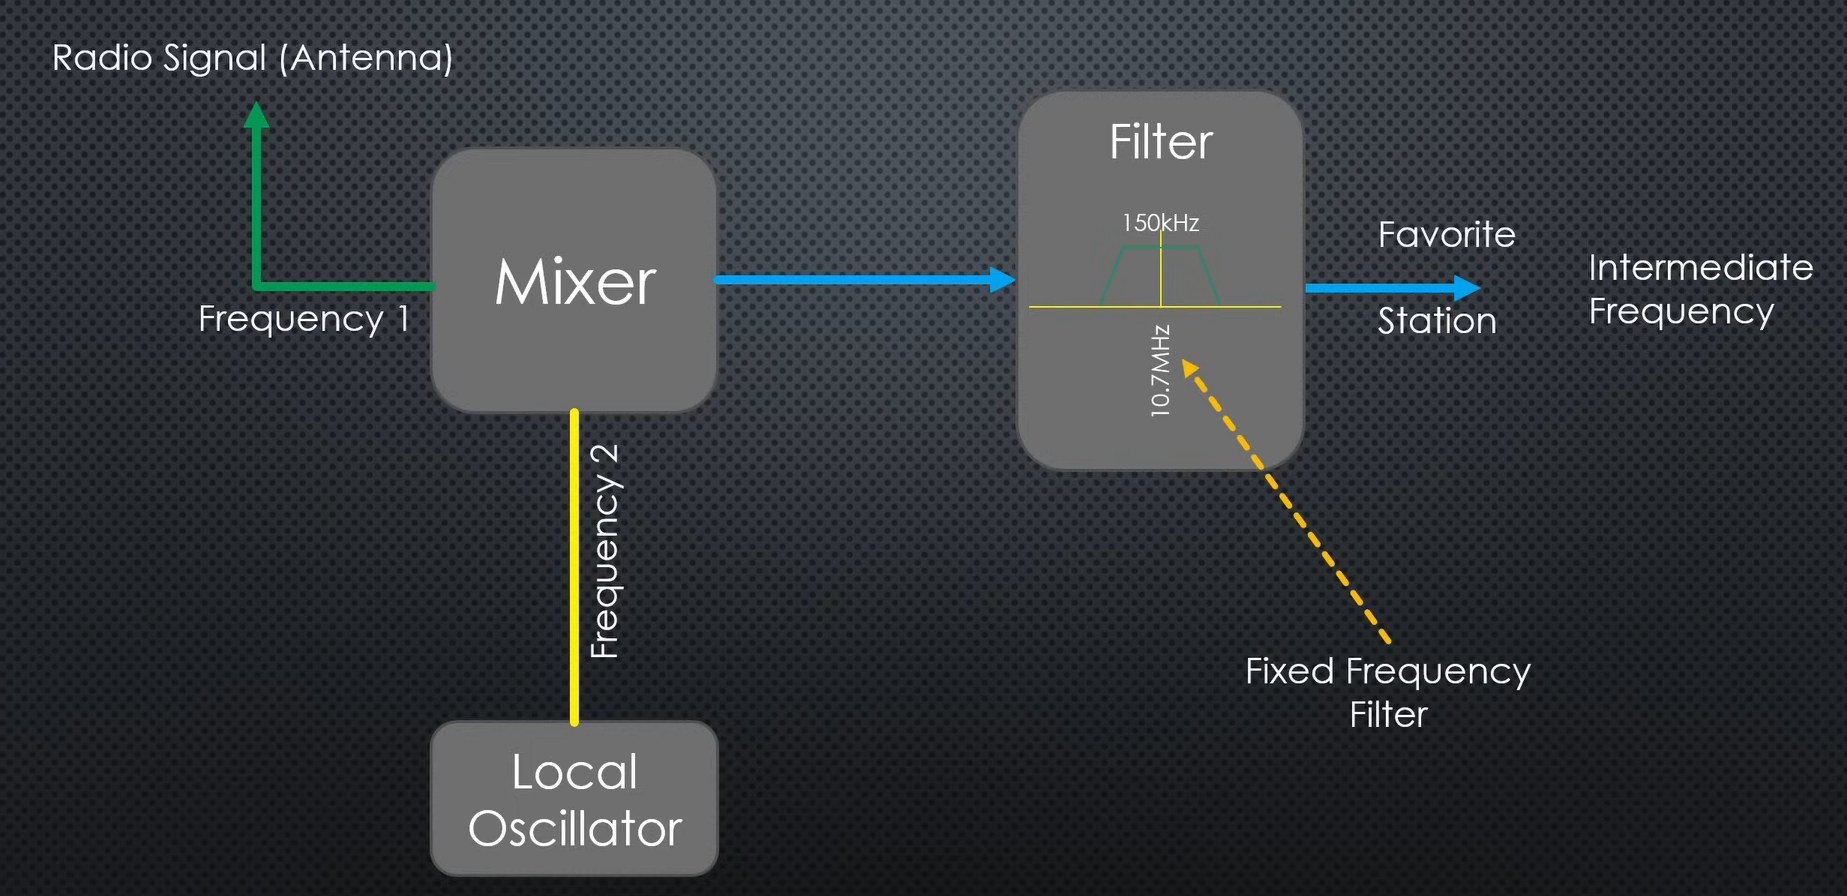
\includegraphics[width=0.85\columnwidth]{Figures/Basics of radio.png}
\caption{Glimse of radio working}
\label{fig:placeholder}
\end{figure}
We uses a Fixed Frequency Filter as they are much cheaper and easier to build.\\

We need Modulators, Demodulators, frequency generators, and Filters for Radio Frequency.
\begin{figure}[H]
    \centering
    \begin{minipage}{0.45\textwidth}
        \centering
        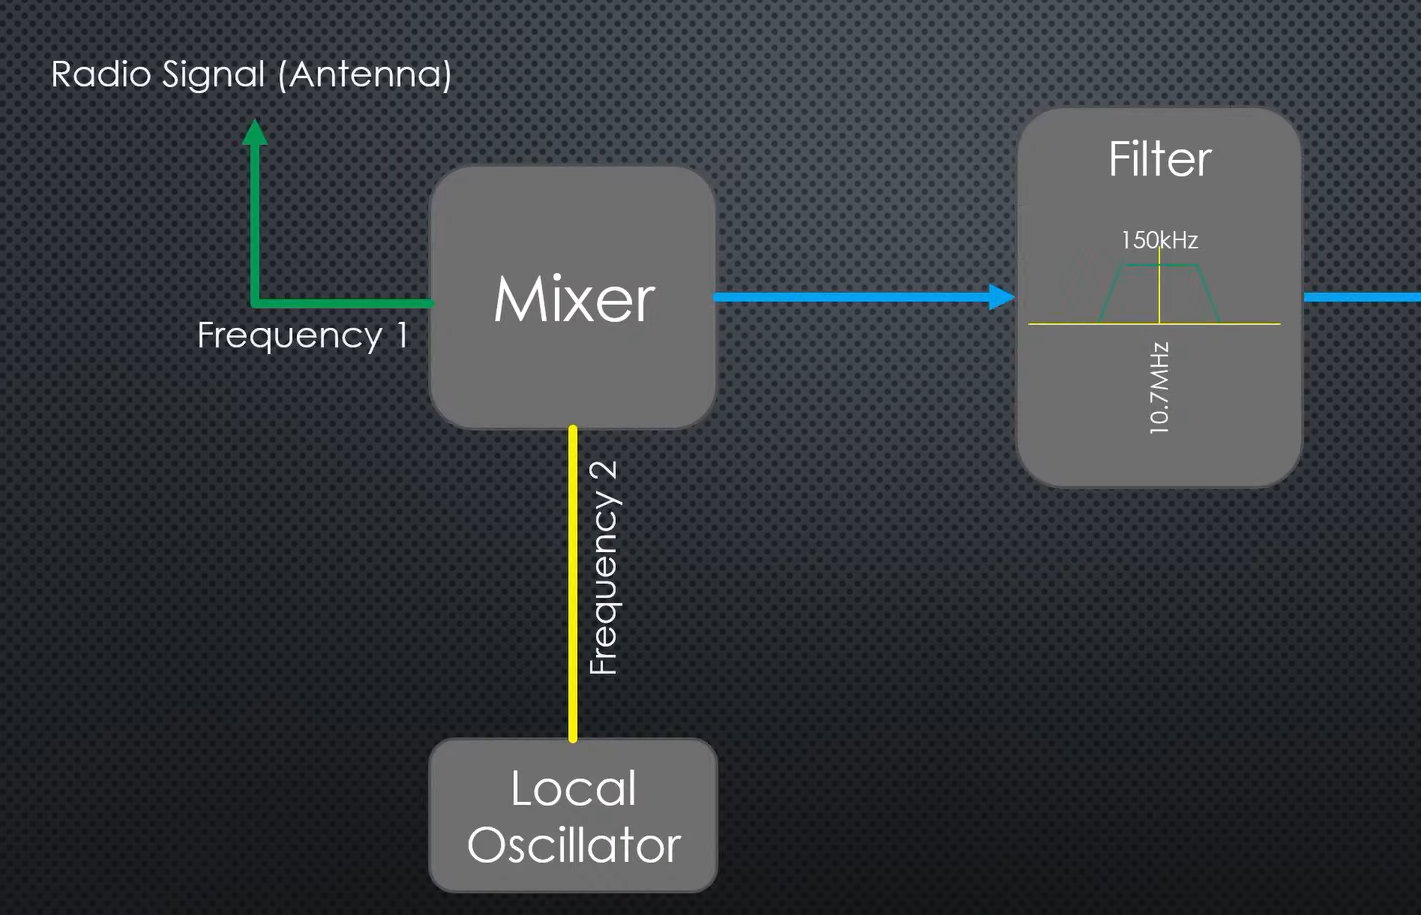
\includegraphics[width=\linewidth]{Figures/What all are needed1.png}
        \caption{Workflow of a radio}
    \end{minipage}
    \hfill
    \begin{minipage}{0.45\textwidth}
        \centering
        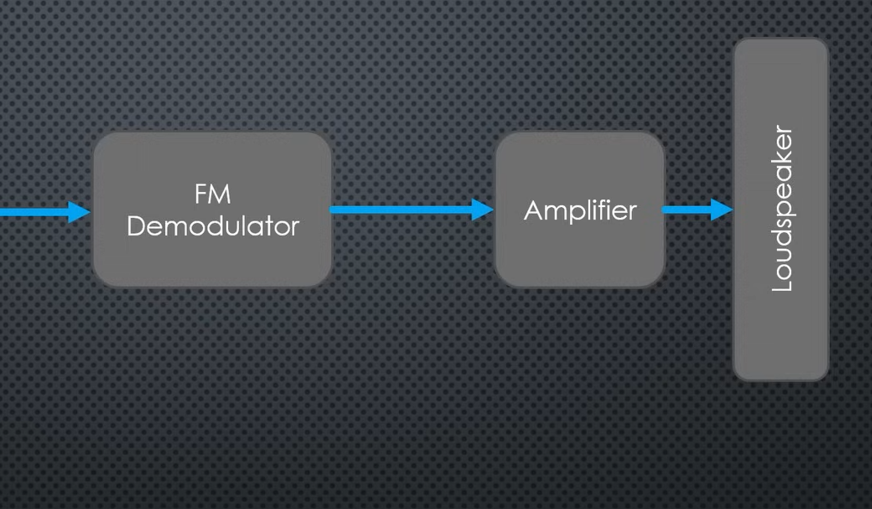
\includegraphics[width=\linewidth]{Figures/continuation.png}
        \caption{}
    \end{minipage}
\end{figure}

\section{Working of RTL-SDR}
\subsection{The Hardware: From Antenna to Digital Data}
The RTL-SDR (Software Defined Radio)
performs three main tasks:

\textbf{Tuning:}\\
It uses a "tuner" chip to focus on a specific frequency (like $100 \text{ MHz}$).\\

\textbf{Down-conversion:}\\
Radio waves vibrate too fast for a computer to process directly. The hardware "shifts" these high frequencies down to a lower, manageable range called Baseband.\\

\textbf{Sampling:}\\
An Analog-to-Digital Converter (ADC) takes "snapshots" of the wave millions of times per second.

\subsection{IQ samples:}
In traditional radio, we only measure the amplitude (height) of a wave. However, waves also have a phase (where they are in their cycle).\\
To capture both, the RTL-SDR splits the signal into two parts:\\
I (In-Phase): The real part of the signal.\\
Q (Quadrature): The imaginary part, which is shifted by $90^\circ$ (one-quarter of a wave).
\begin{figure}[H]
\centering
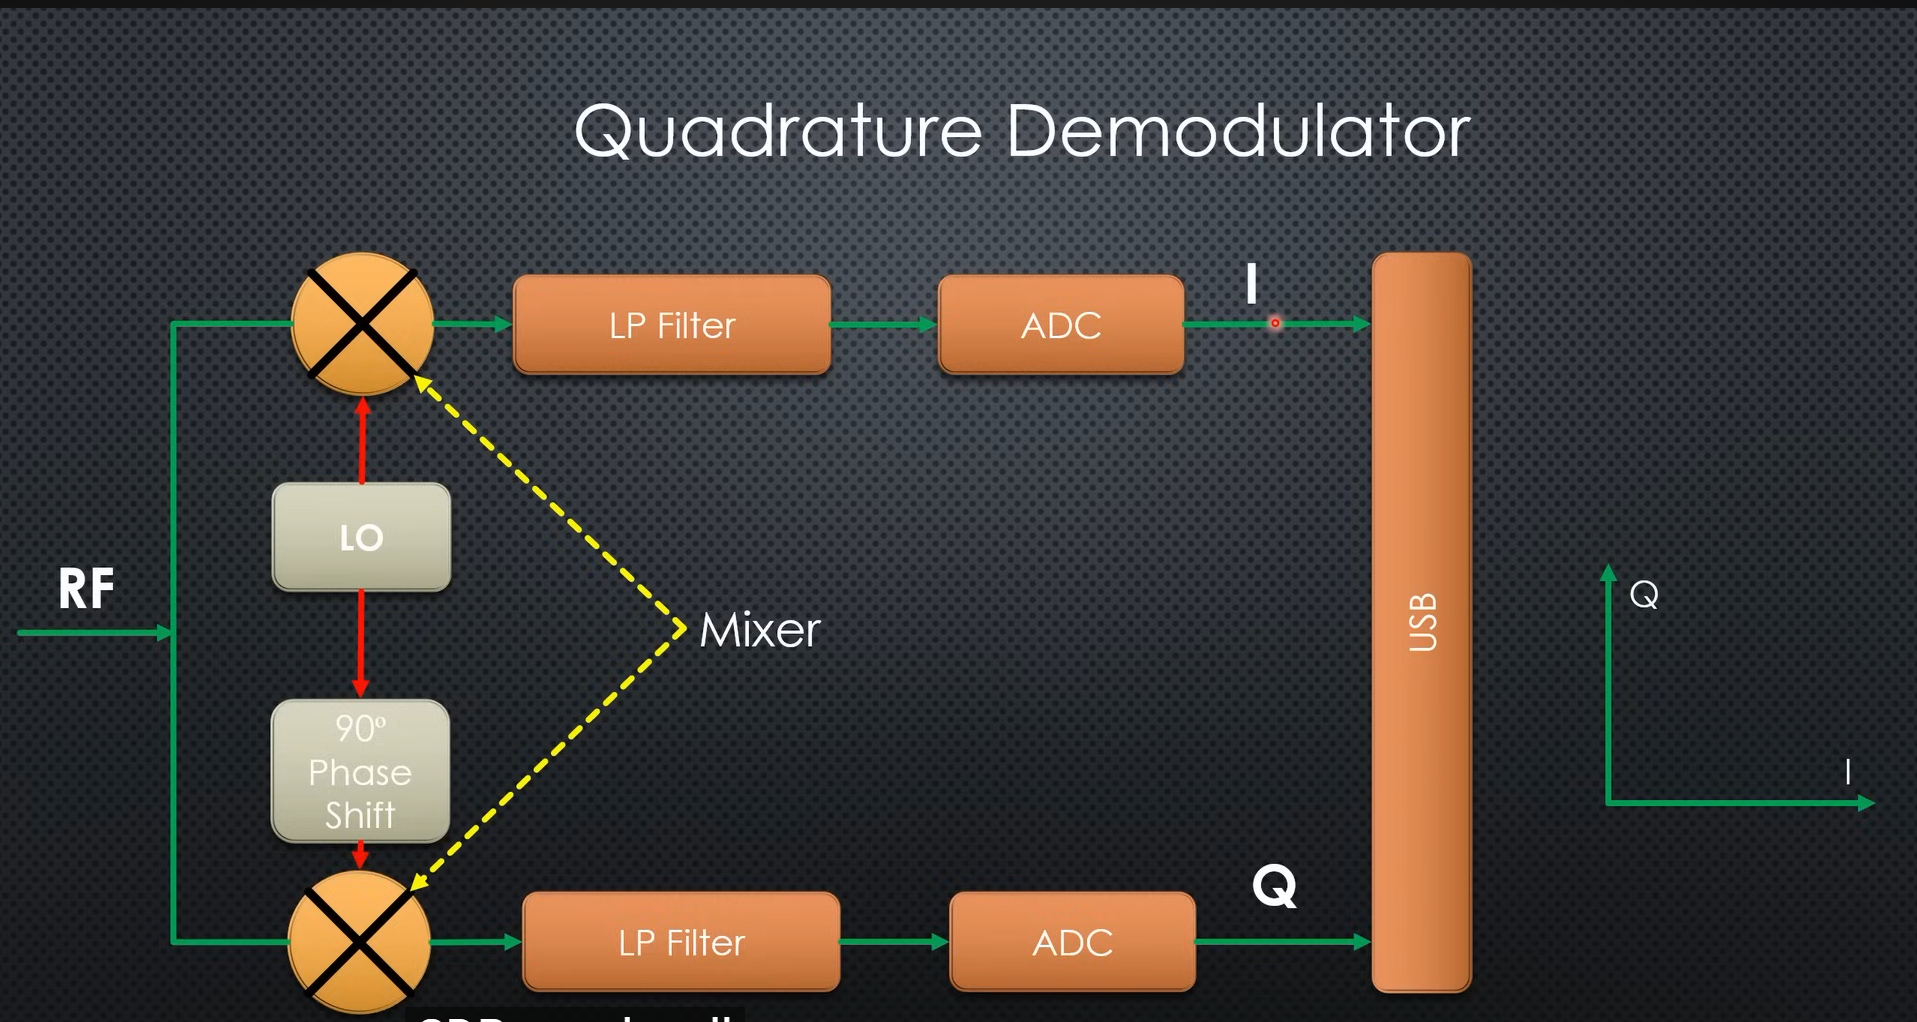
\includegraphics[width=0.75\columnwidth]{Figures/Quadrate Demodulator.png}
\caption{IQ sampling}
\label{fig:placeholder}
\end{figure}
\section{Trying to receive RF using a mobile app}
$\rightarrow$ I tried to listen to Radio signals at a particular frequency, connecting RTL-SDR to my Mobile using an OTG cable and using a mobile app, but it was not clear.\\

$\rightarrow$ then I shifted to GNU Radio using the WSL terminal.
\section{Local Frequency Reception Using GNU Radio}
\subsection{Installation of GNU Radio}

The following commands initialise the Linux environment and the Digital Signal Processing (DSP) stack.\\

 System Update:   
    \begin{center}
        \fbox{\texttt{sudo apt update}}\\
    \end{center}
Dependency Installation:
\begin{center}
    \fbox{\texttt{sudo apt install gnuradio gr-osmosdr rtl-sdr}}
    \end{center}
Install the Audio Bridge:
    \begin{center}
    \fbox{\texttt{sudo apt install libpulse0 pavucontrol
    lsusb}}\\
     \end{center}
Launch Designer:
     \begin{center}
    \fbox{\texttt{gnuradio-companion}}
    \end{center}
\\
For environments where the hardware is not natively accessible (like WSL2), the usbipd toolchain is used to bridge the physical USB bus to the Linux kernel.\\

(The following steps can be ignored for a Native Linux system)\\
    \begin{center}
    \fbox{\texttt{usbipd list}}\\
    \end{center}
    Identifies the Bus ID of the connected RTL-SDR.\\
    \begin{center}
    \fbox{\texttt{usbipd bind --busid <ID>}}\\
     \end{center}
    Shares the hardware with other distributions.\\
    \begin{center}
\fbox{\texttt{usbipd attach --wsl --busid <ID>}}\\
\end{center}
Persistently attaches the device to the WSL2 kernel.\\

\subsection{Digital Signal Processing(DSP) Flow graph}
Here I tried Capturing FM at 98.3M Hz (Radio Mirchi) Frequency.

\begin{figure}[H]
\centering
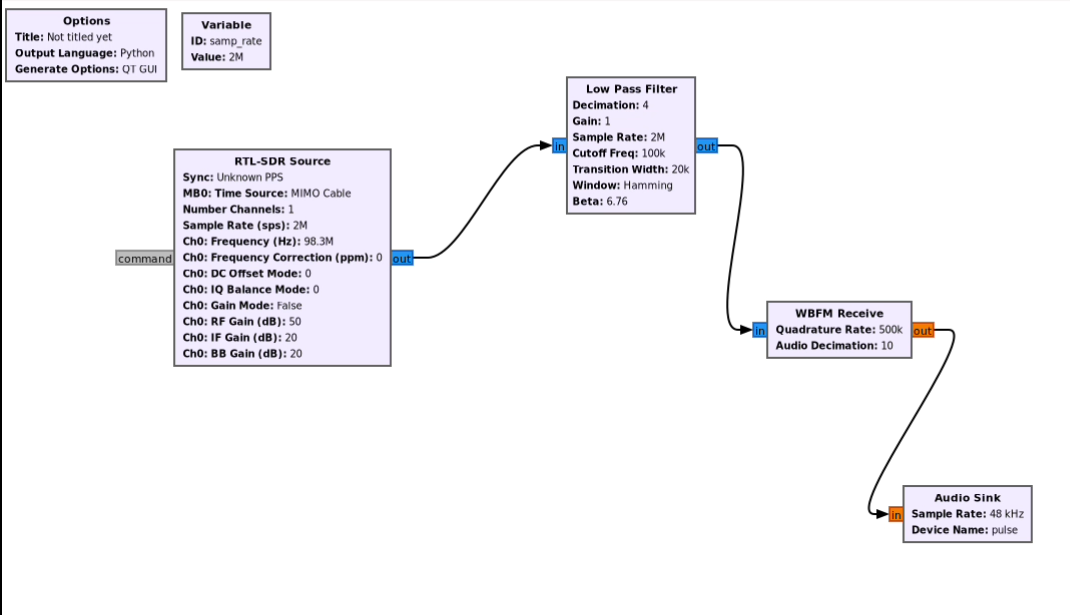
\includegraphics[width=1.0\columnwidth]{Figures/GNU radio at 98.3M Hz(Radio Mirchi).png}
\caption{98.3M Hz (Radio Mirchi)}
\label{fig:placeholder}
\end{figure}
(FM received using GNU radio at 98.3M Hz is available at Videos/FM received at 98.3M Hz(Radio Mirchi).)\\

$\rightarrow$ RTL-SDR Source:\\ Captures raw IQ samples at 2 MHz (samp\_rate).\\

$\rightarrow$ Low Pass Filter:\\ Cleans the signal by removing noise outside the FM channel (100 kHz cutoff).\\

$\rightarrow$ WBFM Receive:\\ The core "math" block that converts the frequency changes into audio.\\

$\rightarrow$ Audio Sink:\\ Sends the final sound to the Windows PulseAudio bridge at 48 kHz.\\

\textbf{Nyquist-Shannon Sampling Theorem:}\\
The theorem states that to accurately reconstruct a signal, the sampling frequency ($f_s$) must be at least twice the highest frequency component ($f_{max}$) of the signal being sampled:
$$f_s > 2 \cdot f_{max}$$
$\rightarrow$ Sampling Rate ($f_s$):\\ 2.0 MHz (Oversampled to ensure Nyquist compliance for the FM band).\\

$\rightarrow$ Audio Interfacing:\\ To bridge the Linux audio stream to Windows hardware, the PulseAudio server was utilised, bypassing traditional ALSA limitations within virtualised environments.\\

\textbf{Software Architecture: .grc \& .py}\\

The files involved in the process:\\

\textbf{The .grc File (The Blueprint):}\\
This is the XML-based configuration file created in GNU Radio Companion.\\ It stores the visual layout of your flowgraph, including the samp\_rate (2 MHz) and the frequency (98.3 MHz).\\

\textbf{The .py File (The Execution):}\\
When you hit the "Play" button, GNU Radio auto-generates a Python script (usually named top\_block.py or FM\_radio.py).
\\
This script uses the Python API to call high-performance C++ libraries to do the heavy math.
\\
You can find this file in your project folder; it is the actual "code" that runs the radio.
\subsection{Observations}
\begin{enumerate}
\item Gain Variation:\\
        Low gain: weak signal, noisy audio\\
        High gain: distortion due to clipping\\
        Optimal gain provided clear reception\\
\item Frequency Offset:\\
    Small frequency mismatch caused audio distortion\\
Correct tuning (98.3 MHz) produced a stable output\\

\item Filter Cutoff Variation:\\
Too narrow: muffled audio\\
Too wide: noisy audio\\
 \item Signal Strength:\\
Indoor reception weaker\\
Antenna orientation affected clarity\\

\item CPU Load:\\
System operated in real-time\\
No major latency observed
    \end{enumerate}

\section{Experimental Validation of RTL-SDR Receiver Using a
Raspberry Pi Based FM Transmitter}
\begin{figure}[H]
\centering
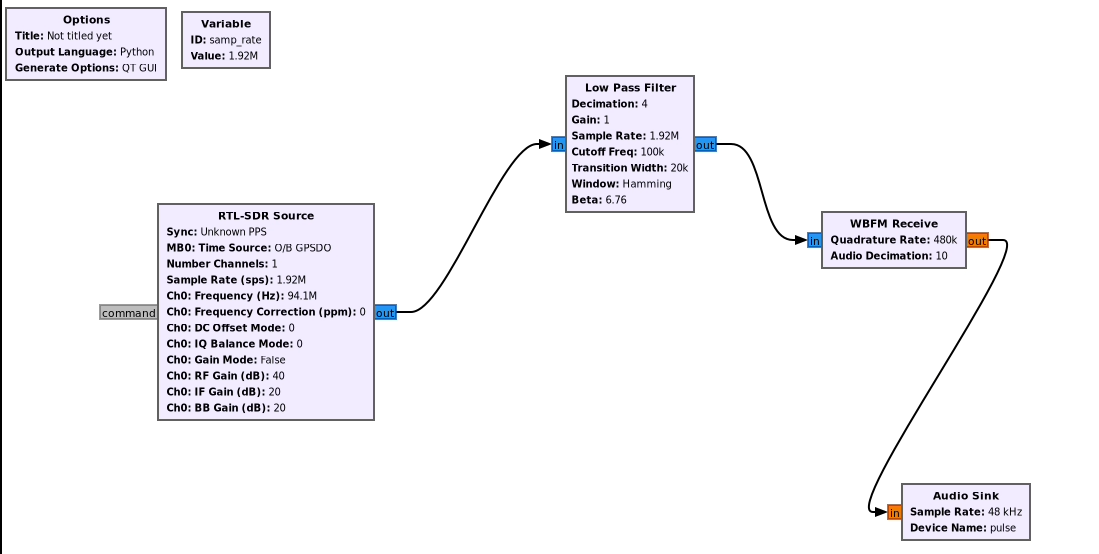
\includegraphics[width=1.0\columnwidth]{Figures/GNU radio at 94.1MHz .png}
\caption{94.1M Hz Transmitted using a Raspbeery Pi}
\label{fig:placeholder}
\end{figure}
(FM received using GNU radio at 94.1M Hz is available at Videos/Received signal sent by Raspberry Pi at 94.1M Hz.)\\

\textbf{Signal Conditioning \& Noise Management:}\\ The Low Pass Filter cutoff was set to 100 kHz with a 20 kHz transition width. This ensures the capture of the full bandwidth of the transmitted signal while still suppressing out-of-band interference.\\

\textbf{Audio Quality:}\\ Initial attempts at a 10 kHz cutoff resulted in high background noise and distorted audio; increasing the bandwidth to 100 kHz significantly improved clarity.\\

\textbf{Hardware Performance:}\\ The RTL-SDR Source gain was maintained at 40 dB to adequately boost the low-power transmission without overloading the receiver.\\

\section{RF Reception Using Python}
The Python code used for this purpose is available at Python/Code.py\\
Can be executed by using the following Commands in WSL terminal\\
(The code is stored in a file named fm\_radio.py):\\
\begin{center}
\fbox{\texttt{chmod +x fm\_radio.py}}\\
\end{center}
\begin{center}
\fbox{\texttt{python3 fm\_radio.py -f 98.3e6 -g 40}}\\
\end{center}
(Frequency and Gain can be varied according to need)
(FM received using Python at 98.3M Hz is available at Videos/Received signal at 98.3M Hz using Python).

\section{Radio Frequency Reception Using Raspberry Pi}
\subsection{Initial Attempt Using RealVNC to Access Raspberry Pi Terminal}

Before achieving a stable setup with Python and SSH, I explored several methods to control the Raspberry Pi. This "trial and error" phase was essential in identifying the power and performance limits of the hardware.\\

\textbf{Initial Attempt: Remote Desktop via RealVNC}\\
My first goal was to operate the Raspberry Pi as if it were a standard desktop computer by using RealVNC Connect.\\

The Plan: Access the Raspberry Pi's graphical "window" (GUI) over the network so I could use visual tools like GNU Radio directly on the Pi.\\

The Obstacle: While the connection was established, the Raspberry Pi's processor was under heavy load trying to render a high-definition desktop while also processing high-speed radio data from the RTL-SDR.
\begin{figure}[H]
\centering
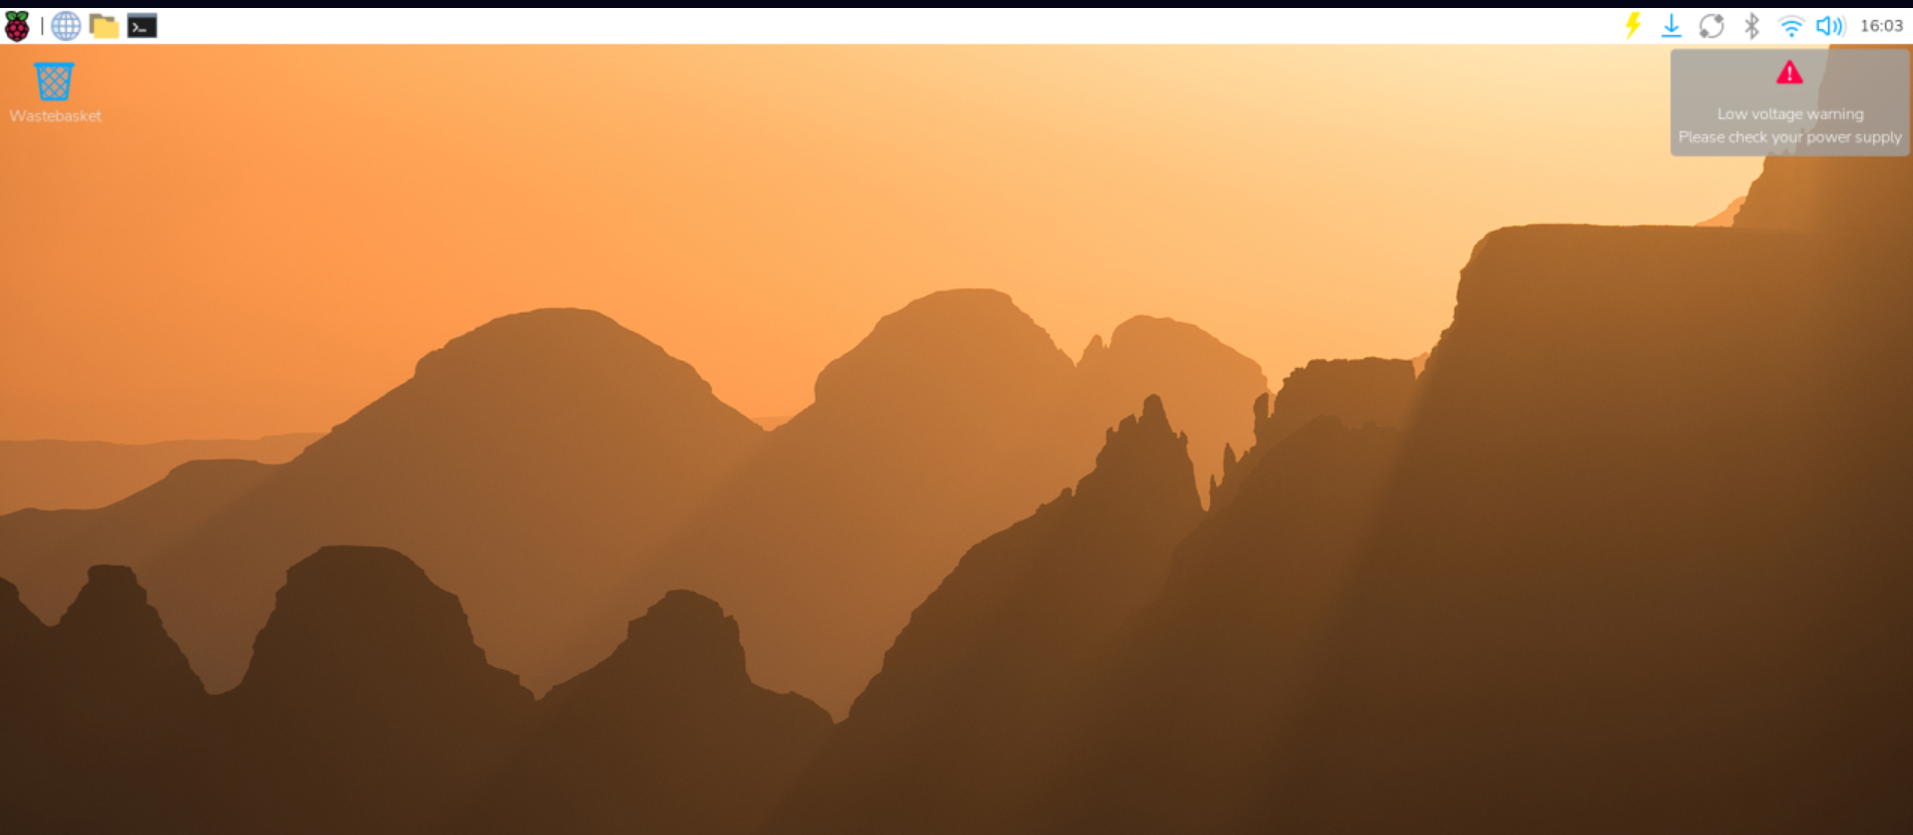
\includegraphics[width=0.75\columnwidth]{Figures/Raspberry Pi Desktop.png}
\caption{Raspbeery Pi Desktop}
\label{fig:placeholder}
\end{figure}

\textbf{The "Low Voltage" Problem}\\
During this phase, the Raspberry Pi displayed a Low Voltage Warning.\\

Diagnosis: The RTL-SDR needed more Power. When combined with the power required to run a full graphical desktop (VNC), the standard power supply could not keep up.\\

Impact: This caused the system to "throttle" (slow down its brain) to save power, leading to dropped radio samples and a laggy interface.\\
I realised that a graphical interface was too "heavy" for this specific portable setup.

\subsection{Accessing Raspberry Pi via SSH from WSL Terminal}
To solve the power and performance issues, I decided to strip away the unnecessary graphical "window" and talk to the Pi using only text-based commands.\\
(This is known as Headless Operation-running a computer without a monitor to save resources.)\\

To ensure the Raspberry Pi could connect to my laptop immediately upon booting, I used Raspberry Pi Imager v2.0.6.\\
This tool allows for "OS Customisation," which injects network and security settings directly into the operating system before the SD card is even inserted into the Pi.\\

Once the SD card was flashed and inserted into the Pi, the following occurred:\\

$\rightarrow$ The Pi powered on and searched for the saved Hotspot SSID.\\
$\rightarrow$My phone (the Hotspot) assigned a dynamic IP Address to the Pi (10.211.129.241).\\
$\rightarrow$On my laptop, I connected to the same Hotspot, placing both devices on the same "Virtual Room" (Local Area Network).\\

Using WSL, I was able to go straight into the Pi using the command and typing the password that was set before:
\begin{center}
\fbox{\texttt{ssh pi@10.211.129.241}}\\
\end{center}
This verified that the pre-configuration was successful, giving me full control over the Pi's terminal without ever needing a physical monitor.\\

Using the following command, I am able to receive the FM signal at the desired frequency and gain:
\begin{center}
\fbox{\texttt{rtl\_fm -f 98.3M -M fm -s 12000 -l 50 -g 40 | aplay -r 12000 -f S16\_LE}}\\
\end{center}
\end{document}
